\section{Datengenerierung}
\label{ch:atengenerierung}

Die Generierung der Daten erfolgt unter Verwendung zweier Normalverteilungen. Dabei werden der Funktion die Mittelwerte sowie die Kovarianzen der Normalverteilungen übergeben.
Anschließend erfolgt eine Zuteilung der Datenpunkte in zwei Klassen. Dazu wird der Richtungsvektor vom ersten Mittelwert zum zweiten Mittelwert berechnet. Dann werden die Datenpunkte, deren Mittelpunkt auf den Koordinatenursprung verschoben wurde, auf den normierten Richtungsvektor projiziert.
Alle Punkte, die nun vor dem Nullpunkt liegen werden der ersten Klasse, jene die nach dem Nullpunkt liegen der zweiten Klasse zugeteilt. Falls die Klassen dadurch unterschiedlich groß werden, wird die Entscheidungsgrenze (in sich vermindernden Schritten) vom Nullpunkt wegbewegt, bis die Klassen gleich groß werden.
Falls die Mittelwerte gleich wären und somit kein Richtungsvektor berechnet werden kann, wird statt diesem der erste Eigenvektor einer PCA verwendet.
Natürlich erfolgt diese Aufteilung der Daten nur, wenn diese linear separierbar sein sollen, falls nicht werden alle Punkte der ersten Normalverteilung der ersten Klasse und jene der zweiten Normalverteilung der zweiten Klasse zugeteilt.

\subsection{Darstellung der Datenvektoren und ihrer Labels als Plot}

\begin{figure}
	
	\centering
	\mbox{
		\subfigure[Leicht separierbare Daten]{
			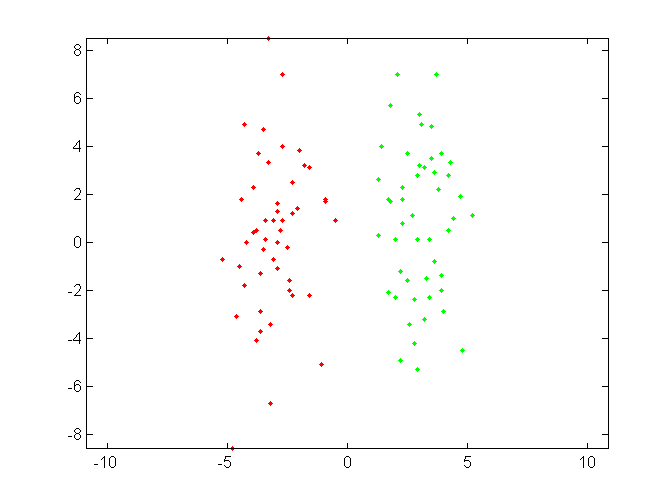
\includegraphics[width=60mm, trim = 0cm 0cm 0cm 0cm]{img/task1simple.png}
		}
		
		\subfigure[Separierbar trotz gleicher Mittelwerte und Kovarianzen]{
			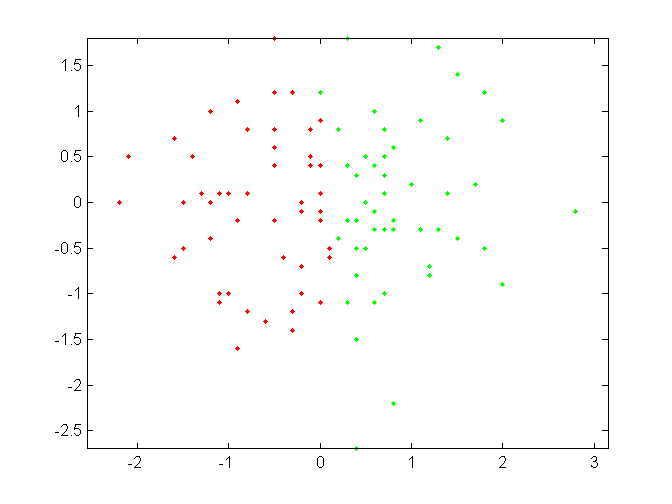
\includegraphics[width=60mm, trim = 0cm 0cm 0cm 0cm]{img/task1close.png}
		}	
	}
	\mbox{
		\subfigure[Nicht linear separierbar]{
			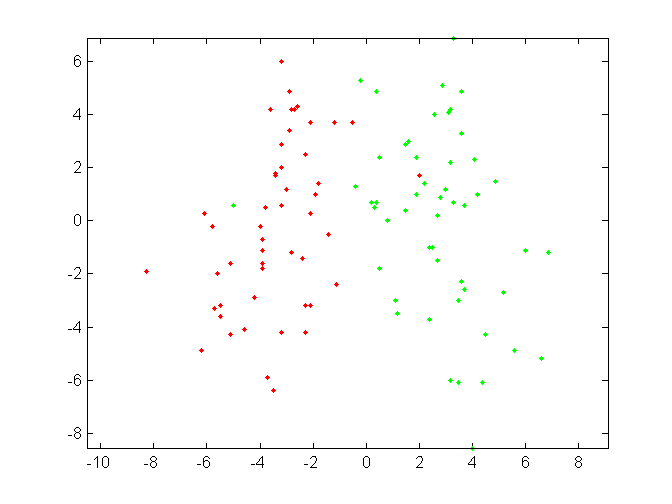
\includegraphics[width=60mm, trim = 0cm 0cm 0cm 0cm]{img/task1notsep.png}
		}
	}
	
	\caption{Darstellung der Datenvektoren und ihrer Labels als Plot}
	\label{fig:gendata}
\end{figure}